\chapter{Introduction}

\textit{This chapter is not finished yet}

\section{WCET Analysis}

In critical systems such as planes and cars it is important that the tasks executed on the hardware meet their deadlines. This is ensured by worst execution time (WCET) analysis. It takes the pair of the program and the dedicated hardware and aims at giving an upper-bound on execution time. 

\TODO{stages of WCET-analysis}

\section{Timing Anomalies}

Phase ordering is a major chellange in WCET-analysis. Most of analysis steps require information from each other (\TODO{examples}), so it is not always possible to order them. 

Nevertheless, most architectures are not composable and contain so-called timing anomalies (TA). Intuitively, TA happens when local worst cases do not constitute a global worst case. TA is observed on the pair of execution traces where the initial hardware state differs, and the instruction sequences are identical. Different cache states can be the source of variation in timing behavior due to miss in one trace and hit in another one.

\begin{example}
Figure \ref{fig:TA1} shows the example of such an anomaly. Here, the assembly sequence consists of 4 instructions ($A,B,C,D$) with data dependencies $A \rightarrow B$ and $C \rightarrow D$. Figure \ref{fig:TA1-trace} represents the pair of traces ($\alpha, \beta$) derived from execution of the given program. There is a variation in latency of instruction $A$ ($1$ in $\alpha$ and $2$ in $\beta$). In trace $\alpha$  the variation is favorable, but the total execution time is also higher in this trace which signals an anomaly.

\label{ex:simple-ta}
\end{example}

\begin{figure}[htbp]
    \centering
    \begin{subfigure}[t]{0.3\textwidth}
        \centering
        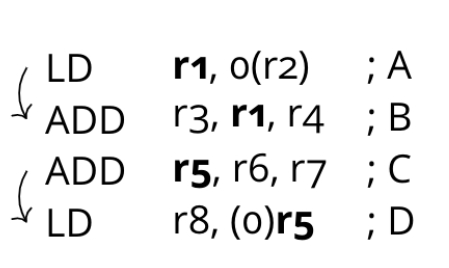
\includegraphics[width=\textwidth]{figures/first-TA-ex-input.png}
        \caption{Inpus assembly sequence}
        \label{fig:TA1-code}
    \end{subfigure}
    \hfill
    \begin{subfigure}[t]{0.55\textwidth}
        \centering
        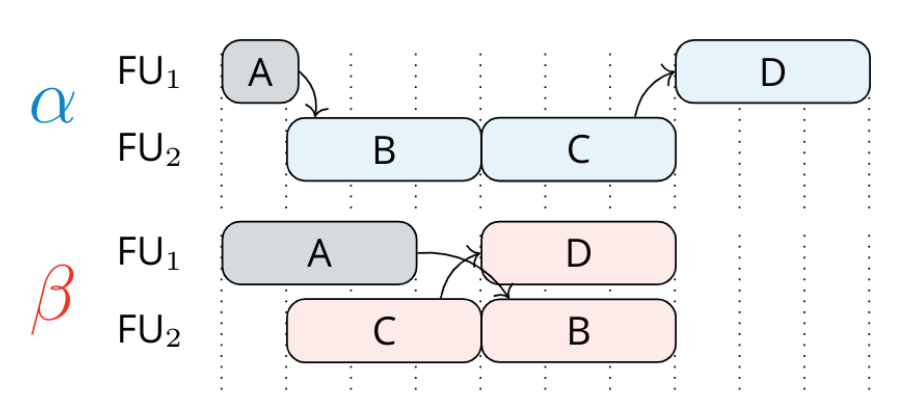
\includegraphics[width=\textwidth]{figures/first-TA-ex-trace.png}
        \caption{Scheduling on functional units comparison}
        \label{fig:TA1-trace}
    \end{subfigure}
    \caption{TA caused by variation in latency of instruction \textit{A} (from \cite{binder_definitions_2022})}
    \label{fig:TA1}
\end{figure}